% !TeX spellcheck = en_US
% !TeX encoding = utf8
% !TeX program = xelatex
% !BIB program = biber 

% \documentclass{beamer}
\documentclass[notes]{beamer}
% \documentclass[draft]{beamer}	
% \usetheme{Singapore}
% \usetheme{Hannover}
\usepackage{pgfpages}
% \setbeameroption{hide notes} % Only slides
% \setbeameroption{show only notes} % Only notes
% \setbeameroption{show notes on second screen=right} % Both

\usepackage[british]{babel}
\usepackage{graphicx,hyperref,url, booktabs}
% \usepackage{ru}
\usepackage{mmstyles}
% \usepackage{hanging}
\usepackage{listings}
\usefonttheme[onlymath]{serif}
\usepackage{fontspec,xunicode}
% \setmainfont{Tahoma}
\usepackage[slantfont,boldfont]{xeCJK}
\setmainfont{Times New Roman}%缺省英文字体.serif是有衬线字体sans serif无衬线字体
\setCJKmainfont[ItalicFont={Adobe Kaiti Std}, BoldFont={Adobe Heiti Std}]{STSong}%衬线字体 缺省中文字体为
\setCJKsansfont{STSong}
\setCJKmonofont{STFangsong}%中文等宽字体

\pgfdeclareimage[width=\paperwidth,height=\paperheight]{bg}{background}
\setbeamertemplate{background}{\pgfuseimage{bg}}

\usepackage[backend=biber]{biblatex}
% \usepackage{biblatex}
\bibliography{./ref.bib}
\addbibresource{ref.bib}

\usepackage{indentfirst}
\usepackage{longtable}
\usepackage{float}
% \usepackage{picins}
\usepackage{rotating}
\usepackage{subfigure}
\usepackage{tabu}
\usepackage{amsmath}
\usepackage{amssymb}
\usepackage{setspace}
\usepackage{amsfonts}
\usepackage{appendix}
\usepackage{listings}
\usepackage{xcolor}
\usepackage{geometry}

%%-----------------------xeCJK下设置中文字体------------------------------%
\setCJKfamilyfont{song}{SimSun}                             %宋体 song
\newcommand{\song}{\CJKfamily{song}}
\setCJKfamilyfont{fs}{FangSong_GB2312}                      %仿宋2312 fs
\newcommand{\fs}{\CJKfamily{fs}}
\setCJKfamilyfont{yh}{Microsoft YaHei}                    %微软雅黑 yh
\newcommand{\yh}{\CJKfamily{yh}}
\setCJKfamilyfont{hei}{SimHei}                              %黑体  hei
\newcommand{\hei}{\CJKfamily{hei}}
\setCJKfamilyfont{hwxh}{STXihei}                                %华文细黑  hwxh
\newcommand{\hwxh}{\CJKfamily{hwxh}}
\setCJKfamilyfont{asong}{Adobe Song Std}                        %Adobe 宋体  asong
\newcommand{\asong}{\CJKfamily{asong}}
\setCJKfamilyfont{ahei}{Adobe Heiti Std}                            %Adobe 黑体  ahei
\newcommand{\ahei}{\CJKfamily{ahei}}
\setCJKfamilyfont{akai}{Adobe Kaiti Std}                            %Adobe 楷体  akai
\newcommand{\akai}{\CJKfamily{akai}}

\newcommand{\verylarge}{\fontsize{60pt}{\baselineskip}\selectfont}  
\newcommand{\chuhao}{\fontsize{44.9pt}{\baselineskip}\selectfont}  
\newcommand{\xiaochu}{\fontsize{38.5pt}{\baselineskip}\selectfont}  
\newcommand{\yihao}{\fontsize{27.8pt}{\baselineskip}\selectfont}  
\newcommand{\xiaoyi}{\fontsize{25.7pt}{\baselineskip}\selectfont}  
\newcommand{\erhao}{\fontsize{23.5pt}{\baselineskip}\selectfont}  
\newcommand{\xiaoerhao}{\fontsize{19.3pt}{\baselineskip}\selectfont} 
\newcommand{\sihao}{\fontsize{14pt}{\baselineskip}\selectfont}      % 字号设置  
\newcommand{\xiaosihao}{\fontsize{12pt}{\baselineskip}\selectfont}  % 字号设置  
\newcommand{\wuhao}{\fontsize{10.5pt}{\baselineskip}\selectfont}    % 字号设置  
\newcommand{\xiaowuhao}{\fontsize{9pt}{\baselineskip}\selectfont}   % 字号设置  
\newcommand{\liuhao}{\fontsize{7.875pt}{\baselineskip}\selectfont}  % 字号设置  
\newcommand{\qihao}{\fontsize{5.25pt}{\baselineskip}\selectfont}    % 字号设置 

\graphicspath{{./fig/}}

% \setbeamertemplate{footnote}{%
%   \hangpara{2em}{1}%
%   \makebox[2em][l]{\insertfootnotemark}\footnotesize\insertfootnotetext\par%
% }

\definecolor{cred}{rgb}{0.6,0,0}
\definecolor{cgreen}{rgb}{0.25,0.5,0.35}
\definecolor{cpurple}{rgb}{0.5,0,0.35}
\definecolor{cdocblue}{rgb}{0.25,0.35,0.75}
\definecolor{cdark}{rgb}{0.95,1.0,1.0}
\lstset{
	language=R,
	numbers=left,
	numberstyle=\tiny\color{black},
	keywordstyle=\color{cpurple}\consolas,
	commentstyle=\color{cgreen}\consolas,
	stringstyle=\color{cred}\consolas,
	frame=single,
	escapeinside=``,
	xleftmargin=1em,
	xrightmargin=1em, 
	backgroundcolor=\color{cdark},
	aboveskip=1em,
	breaklines=true,
	tabsize=3
} 

\makeatletter
\long\def\beamer@author[#1]#2{%
  \def\insertauthor{\def\inst{\beamer@insttitle}\def\and{\beamer@andtitle}%
  \begin{tabular}{rl}#2\end{tabular}}%
  \def\beamer@shortauthor{#1}%
  \ifbeamer@autopdfinfo%
    \def\beamer@andstripped{}%
    \beamer@stripands#1 \and\relax
    {\let\inst=\@gobble\let\thanks=\@gobble\def\and{: }\hypersetup{pdfauthor={\beamer@andstripped}}}
  \fi%
}
\makeatother

% \setbeamersize{text margin left=60mm} 
\setbeamertemplate{frametitle}[default][right]

% The title of the presentation:
%  - first a short version which is visible at the bottom of each slide;
%  - second the full title shown on the title slide;
\title[毕设开题]{\ahei   毕业论文开题答辩}

% Optional: a subtitle to be dispalyed on the title slide
\subtitle{\akai  深度行人再识别学习}

% The author(s) of the presentation:
%  - again first a short version to be displayed at the bottom;
%  - next the full list of authors, which may include contact information;
\author[xinglu]{
	姓名学号: & 王兴路 3140102282 \\
	指导老师: & 李英明 \\
	年级专业: & 2014级信息工程
}
% The institute:
%  - to start the name of the university as displayed on the top of each slide
%    this can be adjusted such that you can also create a Dutch version
%  - next the institute information as displayed on the title slide

\institute[信工1403]{}

% Add a date and possibly the name of the event to the slides
%  - again first a short version to be shown at the bottom of each slide
%  - second the full date and event name for the title slide
\date[\today]{}

\begin{document}

\AtBeginSection[]
{
	\begin{frame}
		\frametitle{大纲}
		\tableofcontents[currentsection]
	\end{frame}
}

% \AtBeginSubsection[2-]
% {
%    \begin{frame}
%        \frametitle{Outline}
%        \tableofcontents[currentsection]
%    \end{frame}
% }

\begin{frame}
	\titlepage
	\note{3月16日下午13:00行政楼108,二次开题答辩,每位同学答辩的时间不少于15分钟(含提问),学生陈述时间为8-10分。

	各组答辩结束后,由各答辩组组长录入开题答辩评语和成绩(接学校最新要求开题成绩有变化),成绩总分30分(文献综述10分、开题报告15分、外文翻译5分),开题不通过(总分低于18分)的学生将参加二次开题答辩。参加二次答辩的学生成绩不高于24分(中等)。}
\end{frame}

\section{背景介绍与研究内容}

% \begin{frame}{test}
% 	\begin{columns}

% 		\column{0.49\textwidth}
% 		This is a text in first column.
% 		$$E=mc^2$$

% 		\column{0.49\textwidth}
% 		This text will be in the second column
% 		and on a second tought this is a nice looking
% 		layout in some cases.
% 	\end{columns}
% \end{frame}


\begin{frame}
	{背景介绍}
	\begin{itemize}
		\item 行人再识别在智能视频监控、智能安防邻域应用广泛
		\item 摄像机网络已广泛布控于各种公共场合中,急需{\hei 跨摄像头}检索行人的技术
		\item 摄像头采集了{\hei 海量}数据,对海量数据进行压缩,建立索引并快速查找
	\end{itemize}
	\begin{figure}
		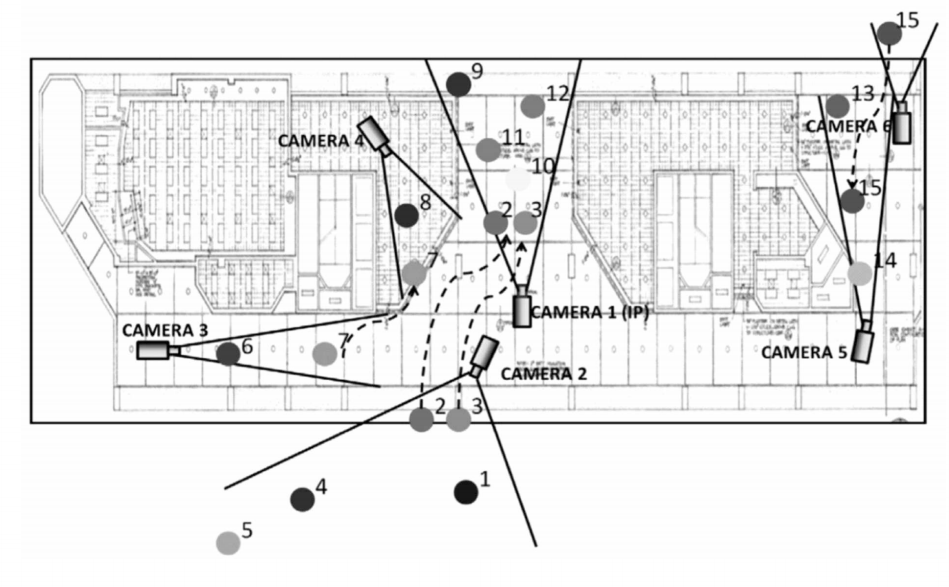
\includegraphics[width=0.75\linewidth]{2018-03-07-19-33-13.png}
	\end{figure}
	\note{
		随着监控摄像机的大规模安装,摄像机网络已广泛布控于各种公共场合中。
		
		利用摄像机网络,我们可以追踪同一行人的轨迹. 但是面对多
		路监控和海量的视频数据,监控人员很容易产生疲惫和应接不暇的状况,我们需要智能视频分析技术弥补人类的不足.
	}
\end{frame}


\begin{frame}
	{行人再识别定义}
	\begin{block}{行人再识别/Person Re-identification/ReID}
	输入某一行人的询问图片(Probe), 在图像或者视频集合(gallery)中跨摄像头检索所有包含该行人的图片. \cite{zheng2016person},\cite{Zheng2017person}
	\end{block}
	\begin{figure}
		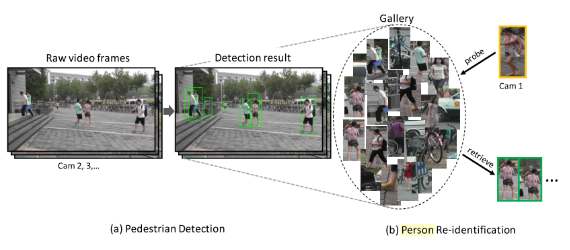
\includegraphics[width=0.9\linewidth]{2018-03-07-19-55-19.png}
	\end{figure}
	\note{目前学者们普遍采用一个简化版本的定义. 这个版本的简化之处在于,他的前提是检测器已经将从图像中检测出行人, 也就是说整个系统的输入是右图的检测后的图片}
\end{frame}
		


\begin{frame}
	{行人再识别定义}
	\begin{block}{行人再识别/Person Re-identification/ReID}
		输入某一行人的询问图片(Probe), 在图像或者视频集合(gallery)中跨摄像头检索所有包含该行人的图片. 
	\end{block}
	\begin{columns}
		\column{0.3\textwidth} 
		\centering 
		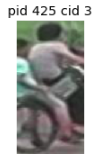
\includegraphics[width=0.5\linewidth]{2018-03-12-10-05-13.png}
		\column{0.7\textwidth} 
		\centering
		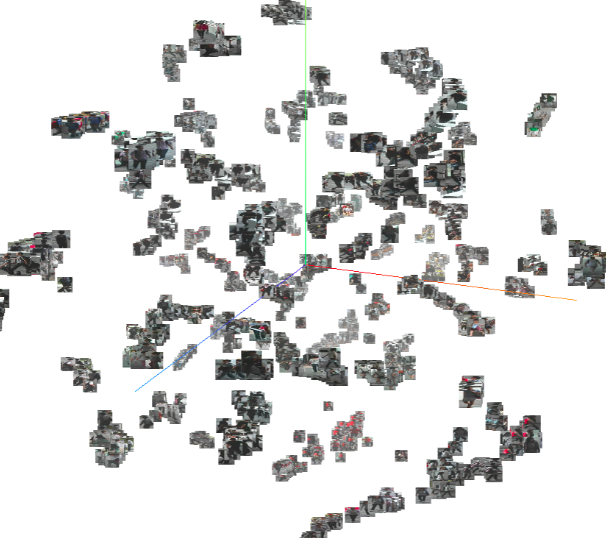
\includegraphics[width=0.72\linewidth]{2018-03-12-09-57-11.png}
	\end{columns}
	\note{
		目前从图像检索的角度来定义, 行人再识别是这样的一个过称...
	比如左图是询问图片, 右图是测试阶段的图像集合
	}
\end{frame}

\begin{frame}
	{行人再识别定义}
	\begin{block}{行人再识别/Person Re-identification/ReID}
		输入某一行人的询问图片(Probe), 在图像或者视频集合(gallery)中跨摄像头检索所有包含该行人的图片. 
	\end{block}
	\begin{figure}
		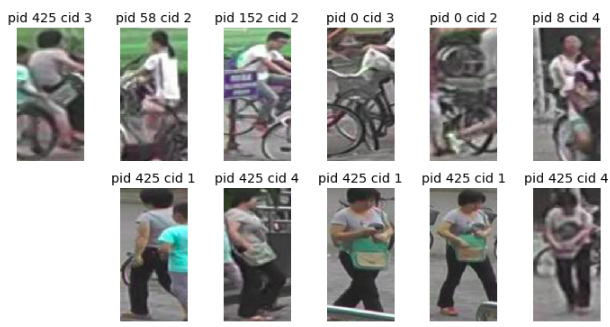
\includegraphics[width=0.9\linewidth]{2018-03-11-22-56-05.png}
	\end{figure}
	\note{右侧第一行是模型的预测结果,第二行是预期的结果. 
	由于询问图片较难, 模型的top-5均预测错误. 
		除了图形检索, 行人再识别还有很多与之相关的领域, 细粒度物体识别 fine-grained classification/少示例大规模分类 few shot extreme classification. 
		
		细粒度物体识别与再识别的联系是,想要区分不同的行人,只能将注意力集中在某些有鉴别力的部位. 
		
		少实例大规模分类与再识别的联系是,再识别有海量的id,每个id的训练样本很少,图片质量通常不好}
\end{frame}


\begin{frame}
	{存在的挑战}
	\begin{description}
		\item[Occlusion] 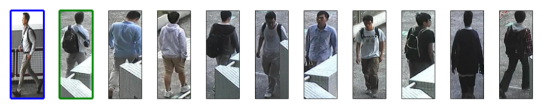
\includegraphics[width=0.9\linewidth]{2018-03-12-10-09-03.png}
		\item[Illumination] 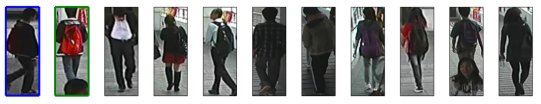
\includegraphics[width=0.9\linewidth]{2018-03-12-10-10-10.png}
		\item[Pose] 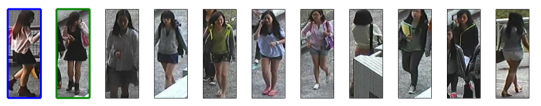
\includegraphics[width=0.9\linewidth]{2018-03-12-10-10-18.png}
		\item[Misalign] 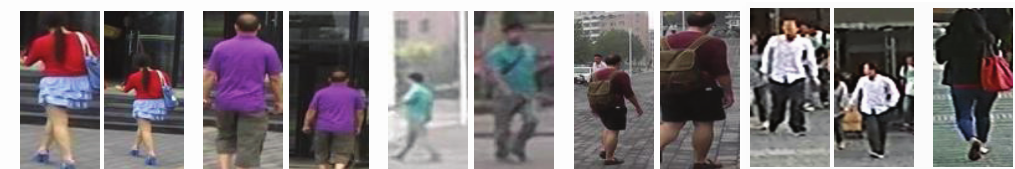
\includegraphics[width=0.88\linewidth]{2018-03-07-20-16-25.png}
	\end{description}
	
	\note{
		
		the learning of comprehensive features of pedestrians for fine-grained tasks remains an open problem.

		 Desired features for open-set FR are expected to satisfy
		the criterion that the maximal intra-class distance is smaller than the minimal inter-class distance under a certain metric space. This
		 由于行人的非刚性运动、检测器的误差、摄像头的
		视角变化,同一行人的不同图片往往存在严重的空间失配(Spatial Misalignment);行
		人没有可靠的生物特征,只能从属性、语义层面的特征加以区分;未标定的摄像机参
		数、巨大的时空跨度,这些都进一步增加了再识别的难度;同时现有的数据集规模相
		对较小,不存在 ImageNet 或者 MegaFace 这样的大规模、可以泛化迁移(Transfer)到
		任意子领域(domain)的数据集。这导致数据集间存在较大偏差(domain bias/domain
		shift),从一个数据集到另一个数据集,
		模型的性能通常都会下降。
	}
\end{frame}

\section{技术路线与设计方案}

\begin{frame}
	{相关工作}
	\begin{itemize}
		\item {\textcolor{blue}{Identification}} 转化为分类问题: 注意力机制提取特征 \cite{liu2017hydraplus}, \cite{zhao2017spindle}, 全局+局部特征 \cite{wei2017glad}
		\item {\textcolor{blue}{Verification}} 转化为两幅图片的验证问题/Verification: \cite{Yaqing2016}
		\item {\textcolor{blue}{Embedding}} 直接学习低维嵌入特征: 在三元损失的基础上强掉难样本的重要性\cite{hermans2017defense}, 全局+局部特征\cite{zhang2017align}, 注意力机制\cite{DBLP:journals/corr/ZhaoLWZ17} 
	\end{itemize}
	\note{主流方法分为三类,采用直接学习embedding的方法,首先介绍采用的baseline方法}
\end{frame}

\begin{frame}
	{基本方法:训练} 
	\begin{itemize}
		\item 特征提取
		\begin{figure}
			\centering
			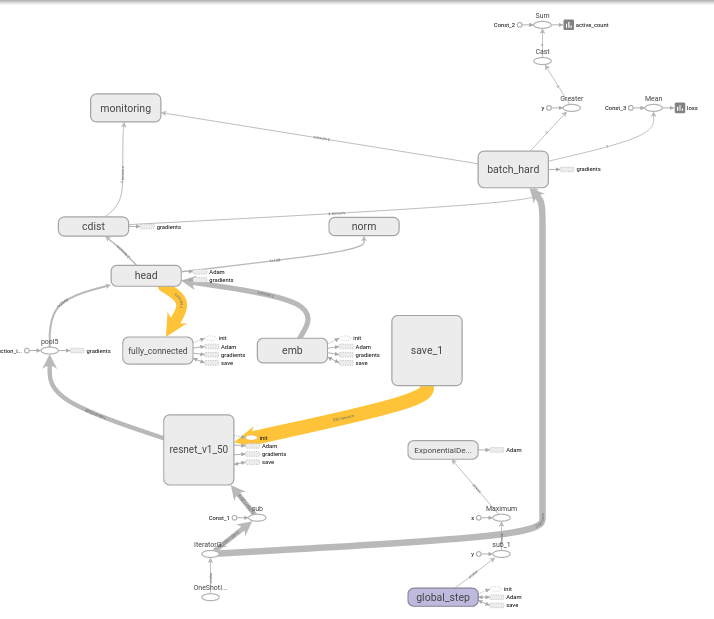
\includegraphics[width=0.82\textwidth]{2018-03-12-10-25-28.png}			
		\end{figure}		
		% \item 难样本挖掘
		% \item 计算损失,反向传播
	\end{itemize}
	% 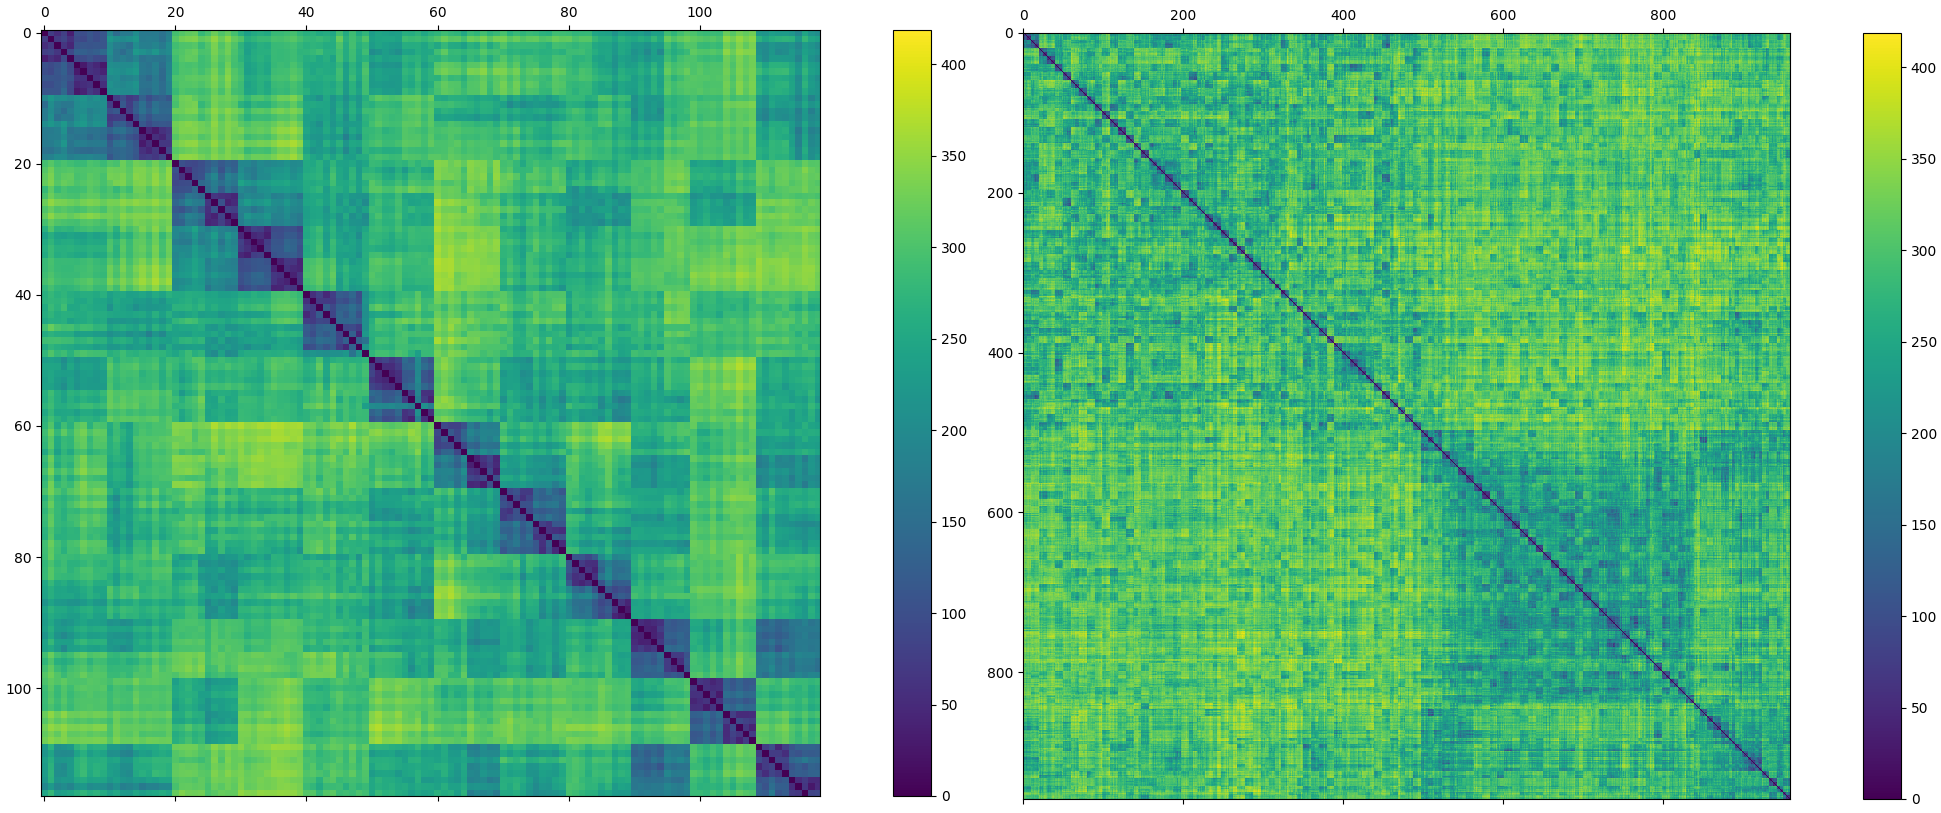
\includegraphics[width=0.7\textwidth]{2018-03-12-10-31-31.png}
	\note{resnet50}
\end{frame}

\begin{frame}
	{基本方法:训练} 
	\begin{itemize}
		\item 特征提取
		% \begin{figure}
		% 	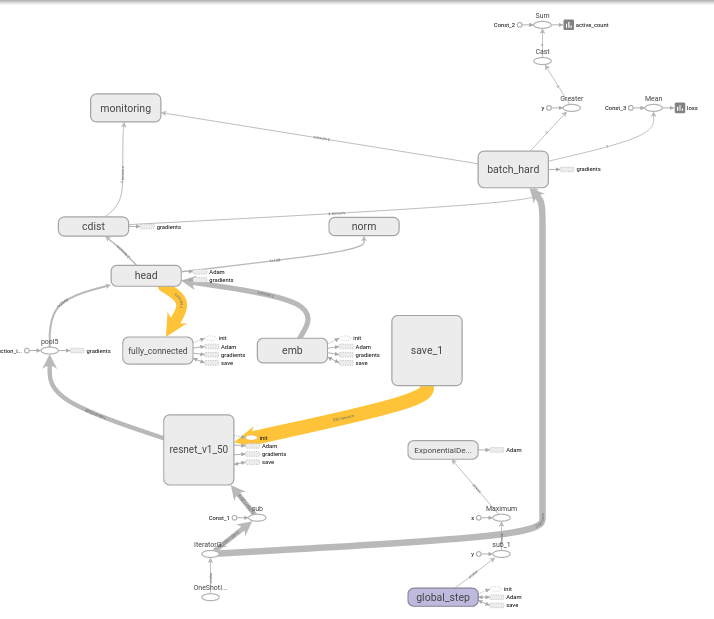
\includegraphics[width=0.7\textwidth]{2018-03-12-10-25-28.png}			
		% \end{figure}		
		\item 难样本挖掘
		% \item 计算损失,反向传播
		\begin{figure}
			\centering
			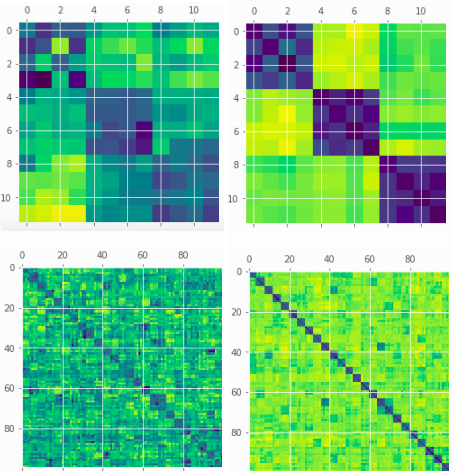
\includegraphics[width=0.65\textwidth]{2018-03-12-14-59-27.png}
		\end{figure}
	\end{itemize}
	\note{分别是什么}
\end{frame}

\begin{frame}
	{基本方法:训练} 
	\begin{itemize}
		\item 特征提取
		\item 难样本挖掘
		\item 计算损失,反向传播
		\begin{equation} 
			L_{tri}=\frac{1}{PK}\sum_{a \in batch} \left( \max_{p \in A} d_{a,p} -  \min_{n \in B} d_{a,n} +\alpha \right)_+
		\end{equation}
	\end{itemize}
	\note{最后计算损失,反向传播}
\end{frame}

\begin{frame}
	{基本方法:测试} 
	\begin{itemize}
		\item 数据增强(随机擦除/多次截取), 特征提取
		\item 计算欧式或余弦距离矩阵
		\item 重排序\cite{zhong2017reranking}, 预测最终排名
	\end{itemize}
	\note{随机擦除,random erasing, 重排序 rerank, 使用}
\end{frame}


\begin{frame}
	{多尺度注意力特征}
	\begin{figure}
		\centering
		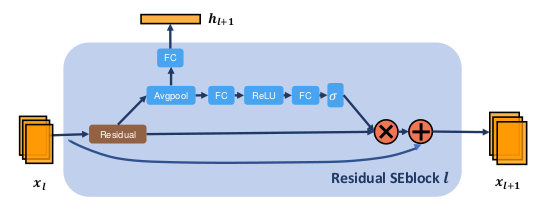
\includegraphics[width=0.78\textwidth]{2018-03-12-11-10-16.png} \\ 
		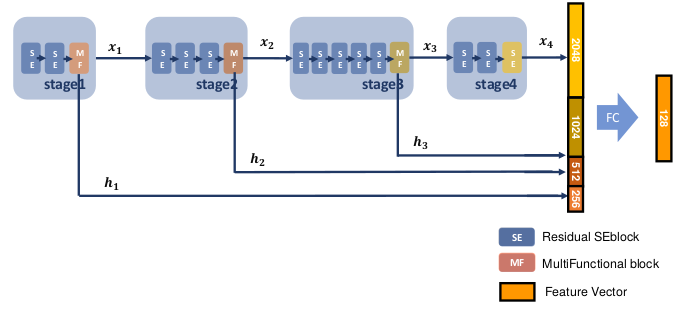
\includegraphics[width=0.89\textwidth]{2018-03-12-11-10-04.png} 
	\end{figure}
	\note{也许是比较小的改进}
\end{frame}

\begin{frame}
	{根据关系图在全局挖掘难样本} 
	\begin{figure}
		\centering 
		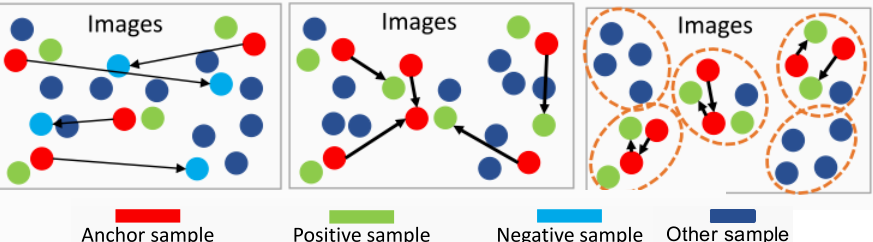
\includegraphics[width=0.9\textwidth]{2018-03-12-11-21-00.png}	
		\caption{不同的形成batch的方法:\textcolor{blue}{左图:}一般的三元损失随机选取三元组,\textcolor{blue}{中图:}\cite{hermans2017defense}在保证一个类至少两个样本的情况下随机选取,\textcolor{blue}{右图:}我们希望在形成batch时难样本就不是随机选取的}
	\end{figure}
	\note{全局挖掘,原来的图是讲什么,我们的方法}
\end{frame}


\section{进度安排与预期目标}
\begin{frame}
	{进度安排}
\begin{table}
	\begin{tabular}{ll}
		\toprule
		2017/11/18--2017/12/18  & 调研文献, 制定规划                                        \\
		2017/12/18--2018/01/19 & 实现基准模型: TriHard \cite{hermans2017defense} \\
		2018/01/19--2018/03/30 & 注意力机制和难样本挖掘的初步探索                                                \\
		2018/03/30--2018/05/16 & 在难样本挖掘方面进一步探索                                                \\
		2018/05/16--2018/06/08 & 撰写毕业论文,答辩                              \\
		\bottomrule
	\end{tabular}
\end{table}
	\note{
		很难说方向一定可行	
	}
\end{frame}

\begin{frame}{现阶段实验}
\begin{table}
	\centering
	\caption{数据集与评估协议的统计信息}
	\label{table:dataset}
	\begin{tabular}{llllll}
		\toprule
		Dataset    & CUHK03 & Market1501 & CUHK01  & DukeMTMC & VIPeR \\
		\midrule
		identities & 1,467  & 1,501      & 971     & 1,812    & 632   \\
		images     & 13,164 & 32,668     & 3,884   & 36,411   & 1,264 \\
		views      & 2      & 6          & 2       & 8        & 2     \\
		train IDs  & 1,367  & 751        & 871/485 & 702      & 316   \\
		test IDs   & 100    & 751        & 100/486 & 1110     & 316   \\
		\bottomrule
	\end{tabular}
\end{table}
\note{需要在各个数据集上验证}
\end{frame}

\begin{frame}{现阶段实验}
	\begin{table}
		\begin{tabular}{lrrr}
			\toprule
			{name} &  top-1 &  top-1.rk &    mAP \\
			\midrule
			cuhk03label.res             &  86.28 &     93.88 &  82.49 \\
			cuhk03label.se.concat       &  89.33 &     96.34 &  86.42 \\
			cuhk03label.se.concat.dop   &  89.83 &     \textbf{97.59} &  86.70 \\
			cuhk03label.res.dop         &  86.84 &     94.66 &  84.18 \\
			cuhk03label.se              &  88.28 &     95.51 &  84.74 \\
			cuhk03detect.res            &  82.79 &     91.11 &  80.08 \\
			cuhk03detect.se.concat      &  84.68 &     91.78 &  81.68 \\
			cuhk03detect.se.concat.dop  &  85.65 &     92.15 &  82.91 \\
			cuhk03detect.se             &  85.50 &     92.84 &  82.78 \\
			cuhk03detect.se.concat.35   &  85.03 &     92.09 &  82.65 \\
			cuhk03detect.se.concat.45   &  85.01 &     92.66 &  82.65 \\
			cuhk03detect.se.sum         &  84.75 &     91.22 &  82.06 \\
			cuhk03detect.se.sum.dop     &  85.93 &     91.53 &  83.21 \\
			cuhk03detect.res.new\_avg    &  83.61 &     90.29 &  81.28 \\
			cuhk03detect.res.dop        &  83.70 &     91.85 &  80.78 \\			
			market1501.res              &  85.61 &     86.12 &  69.53 \\
			market1501.se               &  87.47 &     87.85 &  72.27 \\
			market1501.se.concat        &  87.42 &     87.47 &  72.16 \\
			market1501.se.concat.dop    &  88.53 &     89.40 &  72.86 \\
			market1501.res.dop          &  86.73 &     87.39 &  70.91 \\
			market1501.se.sum           &  87.21 &     87.42 &  71.69 \\
			market1501.se.sum.dop       &  87.70 &     88.06 &  71.95 \\
			\bottomrule
			\end{tabular}
	\end{table}
	\note{只进行了初步实验,并不是都有效果的}
\end{frame}


\begin{frame}[t, allowframebreaks]
\frametitle{References}


\printbibliography
\end{frame}

\begin{frame}
	\chuhao Thank you! %\fontspec{LHANDW.TTF}
\end{frame}


\end{document}
